%==============================================================================
%== template for LATEX poster =================================================
%==============================================================================
%
%--A0 beamer slide-------------------------------------------------------------
\documentclass[final]{beamer}
\usepackage[orientation=landscape,size=a0,
            scale=1.5         % font scale factor
           ]{beamerposter}
           
\geometry{
  hmargin=2.5cm, % little modification of margins
}

%
\usepackage[utf8]{inputenc}

\linespread{1.15}
%
%==The poster style============================================================
\usetheme{sharelatex}
\begin{document}
%==Title, date and authors of the poster=======================================
\title

[BAPG, 6 December 2014, Davis, CA, USA] % Conference
{ % Poster title
ANGSD-wrapper: scripts to streamline and visualize NGS population genetics analysis
}

\author{ % Authors
Arun Durvasula\inst{1}, Tyler Kent\inst{1}, Siddharth Bhadra-Lobo\inst{1}, Jeffrey Ross-Ibarra\inst{2}
}
\institute
[University of California, Davis] % General University
{
\inst{1} Dept. of Plant Sciences, University of California Davis\\[0.3ex]
\inst{2} Dept. of Plant Sciences, Center for Population Biology, and Genome Center, University of California Davis\\[0.3ex]
}
\date{\today}




\begin{frame}[t]
%==============================================================================
\begin{multicols}{3}
%==============================================================================
%==The poster content==========================================================
%==============================================================================

\section{Introduction}

The advent of highly multiplexed sequencing has brought led to the rapid generation of new genomic data. 
One of the powerful approaches enabled by inexpensive sequencing is the ability to sequence a large number of individuals, each to relatively low sequencing depth. 
However, this approach also presents statistical challenges in the analysis of low-coverage data.  The software package ANGSD \ref(Korneliussen).
In order to aid in the analysis of next generation sequencing data, population genetics software such as ANGSD has been developed. This program allows the user to calculate population genetic statistics such as site frequency spectrums, neutrality tests, and 
theta estimators from sequence data aligned to a reference. ANGSD uses likelihood based approaches to make full use of the data afforded by highly multiplexed sequencing. This has been used several studies to calculate summary statistics ( CITATIONS ). However, ANGSD requires much familiarity with command line tools and remains inaccessible to biologists that are not from a computational background. 
	Here we present a software package that aids in the preparation of analysis and facilitates analysis with interactive graphing software implemented in R and Shiny. Before analysis, angsd-wrapper turns a multistep analysis such as calculating Tajima’s D into one step where the information needed is supplied using a configuration file. After ANGSD has finished the calculations, a browser based application can be used to interactively graph the results. 


\section{Implementation}

ANGSD-wrapper is implemented using bash scripts that call ANGSD methods and handle saving intermediate files between the initial data preparation and the final data analysis. 
Each overall method in ANGSD, such as calculating estimates of $\theta$, follows a specific order of program calls. 
Thus, we have abstracted away the running of each step and provided a set of default values for parameters and instead require the user to supply the data using a configuration file (figure 1a). 
The user can override the default values of the parameters in the configuration file as well.
	
Additionally, angsd-wrapper contains a powerful graphing application based on R and Shiny (figure 1b). 
After the analysis is done by ANGSD, the user can load the resulting statistics into a web-based application hosted on the user’s computer. 
This application allows the interactive plotting of values such as estimators of $\theta$ and Tajima’s D as well as the ability to load gene annotations from Ensembl. 
These features make it easy and intuitive to analyze next generation sequencing data. 


\vskip1ex
\begin{figure}
\centering
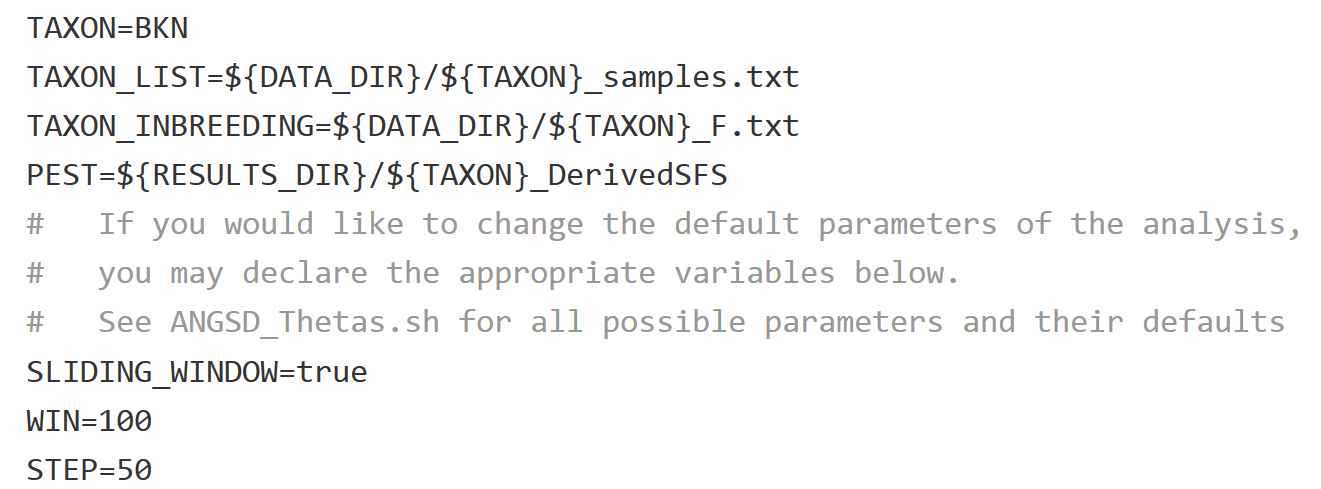
\includegraphics[width=0.99\columnwidth]{conf.png}
\caption{Figure 1a. Example configuration file.}
\end{figure}
\begin{figure}
\centering
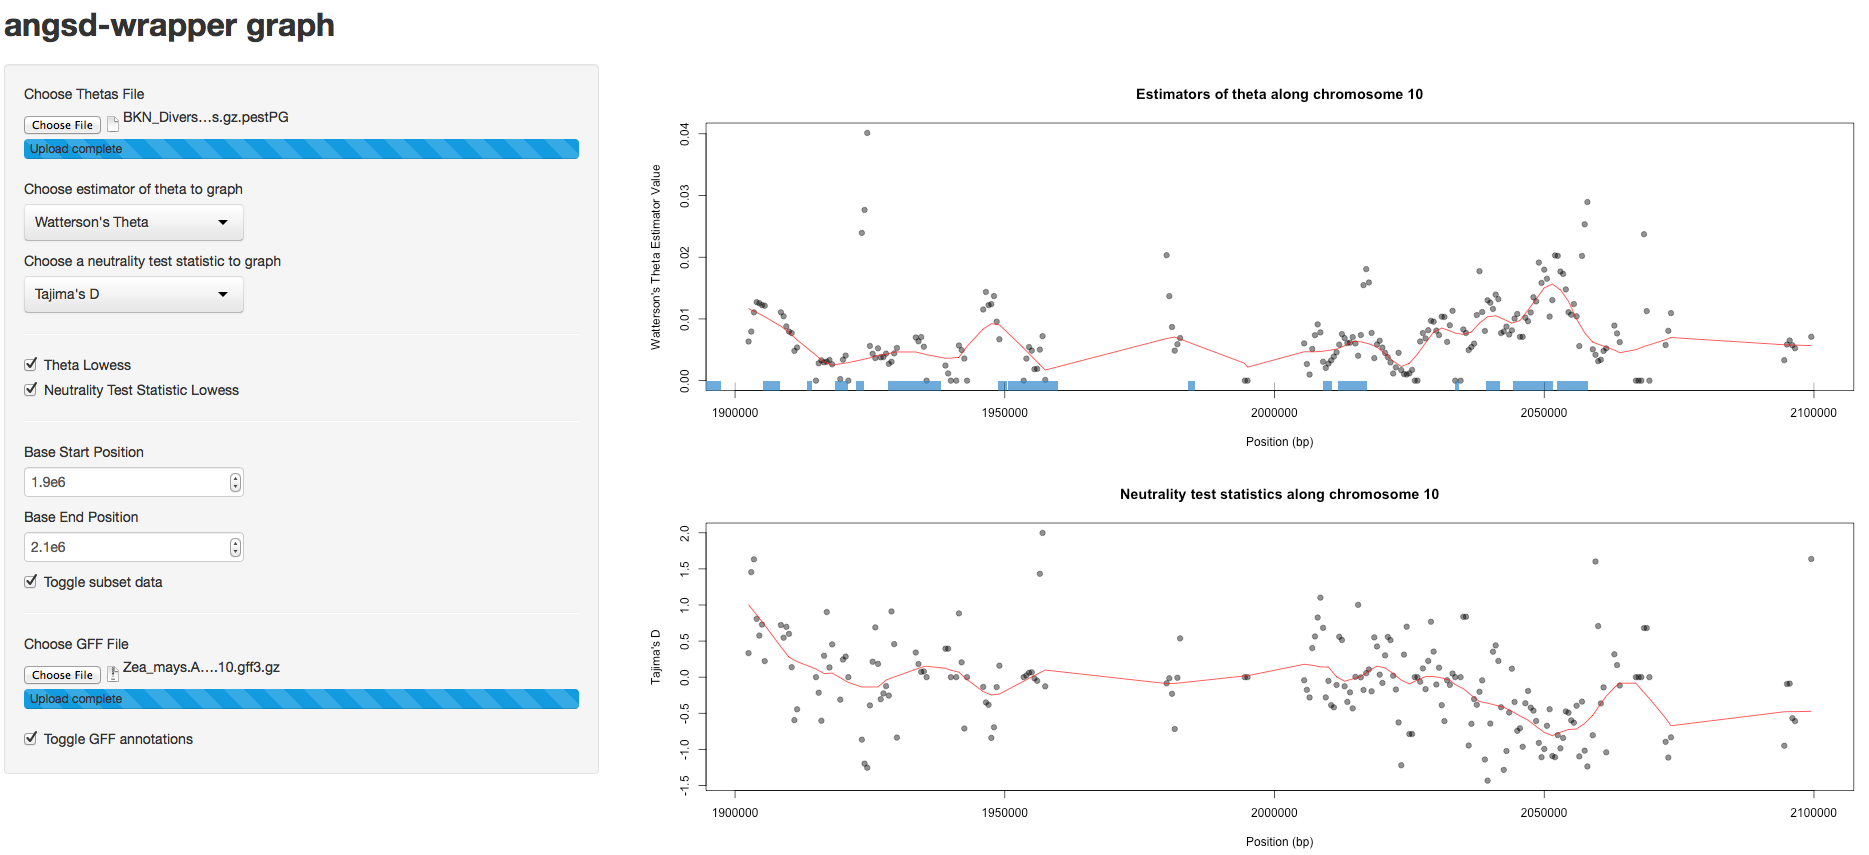
\includegraphics[width=0.99\columnwidth]{screenshot.png}
\caption{Figure 1b. angsd-wrapper interface}
\end{figure}
\vskip2ex

\section{Example Application}

We sequenced 8 genomes of the wild rice \emph{Oryza glumaepatula}, 4 each from populations allopatric and sympatric to cultivated fields of the domesticated \emph{Oryza sativa} ssp. \emph{indica}, in order to investigate evidence of crop-wild introgression. 
\emph{O. glumaepatula} is a potentially endangered species 1.8 MY diverged from domesticated rice \cite{Zhang} native to Central and South America (Vaughan et al. 2003). 
Both species share a AA genome (Vaughan et al. 2003) and we have successfully crossed them experimentally, providing reason to believe the possibility of natural hybridization and thus the risk of wild population decline and extinction (Rhymer & Simberloff 1996). 
Preliminary analysis using angsd-wrapper is suggestive of introgression as evidenced by higher correlation of nculeotid diversity (pi) between domesticated rice and the sympatric population than between domesticated rice and allopatric O. glumaepatula (Fig. 2).

%make this a caption on the figure
\vskip1ex
\begin{figure}
\centering
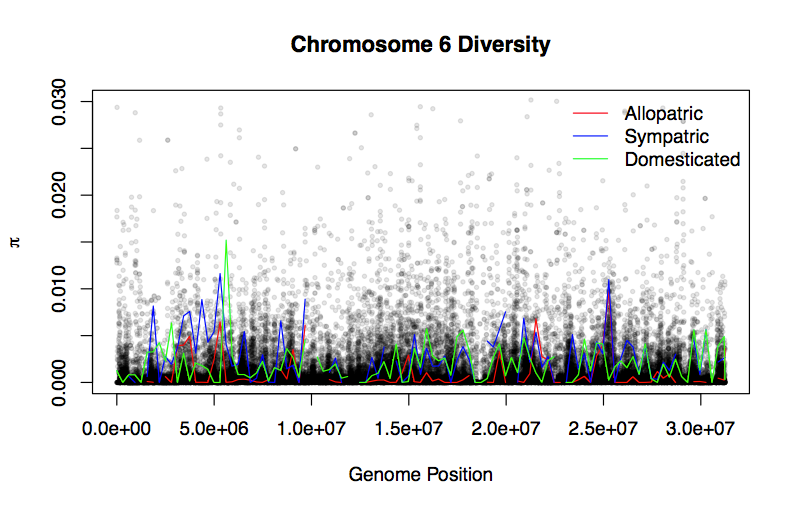
\includegraphics[width=0.99\columnwidth]{chr6rice.png}
\caption{Figure 2. Nucleotide diversity ($\pi$) along chromosome 6.  
Correlation of pi between domesticated rice and the sympatric population is 0.417, while between domesticated rice and the allopatric population it is 0.077.}
\end{figure}
\vskip2ex




%==============================================================================
%==End of content==============================================================
%==============================================================================

%--References------------------------------------------------------------------

\section{References}

\begin{thebibliography}{99}

\bibitem{Akimoto} Akimoto M, Shimamoto Y and Morishima H (1998). Mol Ecol 7:1371-1381.

%Buso GSG, Rangel PH and Ferreira ME (2001). Mol Ecol 7:107-117.
%Ge S, Oliveira GCX, Schaal BA, Gao LZ and Hong DY (1999) RAPD variation within and between natural populations of the 	wild rice Oryza rufipogan from China and Brazil. Heredity 82:1-7.
%Karasawa, M. M. G., et al. (2007). "Genetic structure of Brazilian wild rice (Oryza glumaepatula Steud., Poaceae) populations 	analyzed using microsatellite markers.” Genetics and Molecular Biology 30: 400-410.
%
%Oka HI (1988) Origin of Cultivated Rice. Japan Scientific Societies Press, Tokyo, and Elsevier Science Publishers, Amsterdam, 	254 pp.
%R Core Team (2014). R: A language and environment for statistical computing. R Foundation for Statistical Computing, 	Vienna, Austria. URL .
%RStudio and Inc. (2014). shiny: Web Application Framework for R. R package version 0.10.2.1. http://CRAN.R-project.org/	package=shiny

\bibitem{Korneliussen} Korneliussen et al. (2014). BMC Bioinformatics. 15:356

\bibitem{R} R Core Team (2014). R Foundation for Statistical Computing, Vienna, Austria \url{http://www.R-project.org/}

\bibitem{Zhang} Zhang Q-J, et al. (2014). PNAS 111:E4954-E4962.

Ryhmer JM and Simberloff D (1996) Extinction by Hybridization and Introgression. Annu Rev Ecol Syst 27:83-109.

Vaughan DA, Morishima H, and Kadowaki K (2003) Diversity in the Oryza genus. Current Opinion in Plant Biology 6:139-146.

\end{thebibliography}
%--End of references-----------------------------------------------------------

\end{multicols}

%==============================================================================
\end{frame}
\end{document}
